In this section, we describe the implementation of the calculation of
interactions in FDPS. Conceptually, it consists of the following two
steps. In the first step, each process determines, for each of other
processes, which of its particles and superparticles are required by
that process for interaction calculation, and sends them to it. In the
second step, each process calculates the interactions onto
$i$-particles by calling user-defined function objects.

\if 0
\begin{enumerate}
\item Each process determines, for each of other processes, which of
  its particles and   superparticles are required by that process for
  interaction calculation,   and sends them to it.

%%
\item Each process calculates the interactions onto  $i$-particles by
  calling user-defined function objects.
\end{enumerate}
\fi

\begin{figure}
  \begin{center}
%    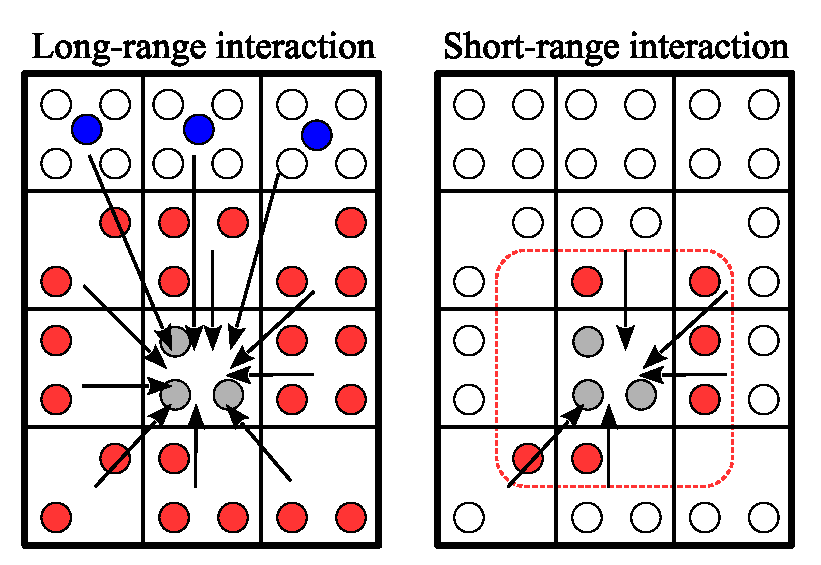
\includegraphics[width=8cm]{fig/exchangeLET.eps}
    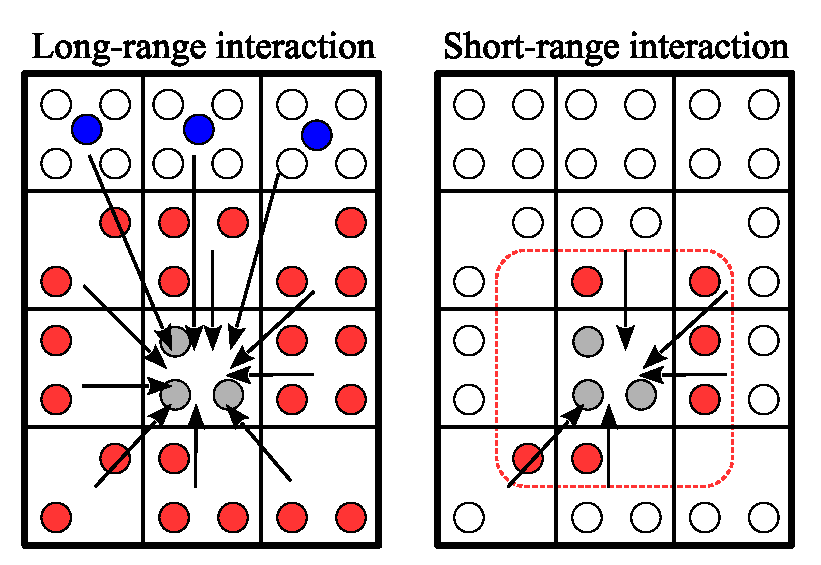
\includegraphics[width=7.5cm]{fig/exchangeLET.eps}
  \end{center}
  \caption{Illustration of communication among processes during the
    interaction calculation.}
  \label{fig:exchangeLET}
\end{figure}

For both steps, the octree structure is used, both for long- and
short-range interactions.
%%In step 1, 
In the first step, each process constructs the tree structure for its
local particles, and uses it to determine what data should be sent to
other processes. For the long-range interactions, this part is done
through the usual tree traversal \cite{1986Natur.324..446B,
  1990JCoPh..87..161B}. For the short-range interactions, tree
traversal is also used. A cube in a tree need to be subdivided if it
is within the cutoff length from anywhere in the domain of the process
to which the data will be sent.  The current implementation of FDPS
can handle four different types of the cutoff length for the
``short-range'' interaction: fixed, $j$-dependent, $i$-dependent and
symmetric.  For $i$-dependent and symmetric cutoffs, FDPS does the
tree traversal twice.  Figure~\ref{fig:exchangeLET} illustrates what
data are sent, for both long- and short-range interactions.

After a process receives all data it requires, it reconstructs the
tree structure which contains all information necessary to calculate
interactions on its particles.

The interaction calculation is performed using this new tree. The
procedure is the same as described in detail in the literature
\cite{1990JCoPh..87..161B, 1991PASJ...43..859M}, except for the
following two differences.  First, this part is fully multithreaded
using OpenMP, to achieve very good parallel performance. Second, for
the interaction calculation the user-provided functions are used, to
achieve the flexibility and high performance at the same time.

% LocalWords:  FDPS TreeForForceLong TreeForForceShort calcForceAllAndWriteBack
% LocalWords:  subdomains substeps octree multipole superparticles nd OpenMP
% LocalWords:  substep multithreading multithreaded
